\documentclass[11 pt]{article}

\usepackage{amsfonts}
\usepackage{amsmath}
\usepackage{fancyhdr}
\usepackage[left=2cm,right=2cm,top=2cm,bottom=2cm]{geometry}
\usepackage{graphicx}
\usepackage[hidelinks]{hyperref}
\usepackage{listings}
\usepackage{subfig}
\usepackage{xcolor}

\pagestyle{fancy}
\fancyhf{}
\lhead{Theoretical Statistical Physics}
\chead{Exercise 07}
\rhead{E. Dizer, V. Mader}
\setlength{\headheight}{15pt}

\newcommand{\pder}[2]{\frac{\partial #1}{\partial #2}} % total derivative
\newcommand{\tder}[2]{\frac{\dd #1}{\dd #2}} % partial derivative
\newcommand{\dd}{\mathrm{d}}
\newcommand{\red}[1]{\textcolor{red}{#1}} 
\newcommand{\blue}[1]{\textcolor{blue}{#1}} 
\newcommand{\green}[1]{\textcolor{green}{#1}} 

\definecolor{commentsColor}{rgb}{0.497495, 0.497587, 0.497464}
\definecolor{keywordsColor}{rgb}{0.000000, 0.000000, 0.635294}
\definecolor{stringColor}{rgb}{0.558215, 0.000000, 0.135316}
\lstset{ %
    backgroundcolor=\color{white},   % choose the background color; you must add \usepackage{color} or \usepackage{xcolor}
    basicstyle=\footnotesize,        % the size of the fonts that are used for the code
    breakatwhitespace=false,         % sets if automatic breaks should only happen at whitespace
    breaklines=true,                 % sets automatic line breaking
    captionpos=b,                    % sets the caption-position to bottom
    commentstyle=\color{commentsColor}\textit,    % comment style
    deletekeywords={...},            % if you want to delete keywords from the given language
    escapeinside={\%*}{*)},          % if you want to add LaTeX within your code
    extendedchars=true,              % lets you use non-ASCII characters; for 8-bits encodings only, does not work with UTF-8
    frame=tb,	                   	   % adds a frame around the code
    keepspaces=true,                 % keeps spaces in text, useful for keeping indentation of code (possibly needs columns=flexible)
    keywordstyle=\color{keywordsColor}\bfseries,       % keyword style
    language=Python,                 % the language of the code (can be overrided per snippet)
    otherkeywords={*,...},           % if you want to add more keywords to the set
    numbers=left,                    % where to put the line-numbers; possible values are (none, left, right)
    numbersep=5pt,                   % how far the line-numbers are from the code
    numberstyle=\tiny\color{commentsColor}, % the style that is used for the line-numbers
    rulecolor=\color{black},         % if not set, the frame-color may be changed on line-breaks within not-black text (e.g. comments (green here))
    showspaces=false,                % show spaces everywhere adding particular underscores; it overrides 'showstringspaces'
    showstringspaces=false,          % underline spaces within strings only
    showtabs=false,                  % show tabs within strings adding particular underscores
    stepnumber=1,                    % the step between two line-numbers. If it's 1, each line will be numbered
    stringstyle=\color{stringColor}, % string literal style
    tabsize=2,	                   % sets default tabsize to 2 spaces
    title=\lstname,                  % show the filename of files included with \lstinputlisting; also try caption instead of title
    columns=fixed                    % Using fixed column width (for e.g. nice alignment)
}


\begin{document}

	%%%%%%%%%%%% GENERAL REMARK %%%%%%%%%%%%%%%%%%%%%%%%%%%%%%%%%%%%
	%%%  A lot of our exercises are taken from:
	%%%  https://mtdevans.com/projects/physics-problems/index.html
	%%%%%%%%%%%%%%%%%%%%%%%%%%%%%%%%%%%%%%%%%%%%%%%%%%%%%%%%%%%%%%%%

    \section{Including optical phonons in the Debye model
        \textit{(5 points)}
    }
    As a classical model for paramagnetism one 
can consider a system of $N$ particles with 
the Hamiltonian
\begin{equation}
    \mathcal{H}=-hM
    \ \ \ \textnormal{with}\ \ \ 
    M=\mu\cdot\sum_{i=1}^N\cos\theta_i
\end{equation}
where $h$ is an external homogeneous magnetic 
field, $\mu$ the magnetic moment of a single 
particle and $\theta_i$ the angle between the
magnetic field $h$ and the magnetic moment
$\mu$ of particle $i$.

\paragraph{1. Use the canonical distribution 
    to calculate the average magnetization, 
    $\langle M\rangle$, as a function of $h$
    and temperature $T$. 
    \textit{(3 points)}
} \ \\
    \\
    Partition function:
    \begin{align}
        Z
        &=\frac{1}{h^{3N}}\cdot
        \int d^{3N}r 
        \int d^{3N}p
        \int d^N\Omega\
        e^{-\beta\mathcal{H}} \\
        &=Z_0\cdot\bigg(
            \int_0^{2\pi}d\varphi 
            \int_0^\pi d\theta
            \cdot\sin\theta\cdot 
            e^{h\beta\mu\sum_i^N\cos\theta_i}
        \bigg) \\
        &=Z_0\cdot\bigg(
            \int_0^{2\pi}d\varphi 
            \int_0^\pi d\theta
            \cdot\sin\theta\cdot 
            e^{h\beta\mu\cos\theta}
    \bigg)^N \\
        &=Z_0\cdot\bigg(
            \frac{4\pi\cdot\sinh(\beta\mu h)}
            {\beta\mu h}
        \bigg)^N
    \end{align}
    Free energy:
    \begin{align}
        F
        &=-k_BT\ln(Z) \\
        &=-k_BT\cdot(\ln(Z_0)+N\ln(4\pi))
        -Nk_BT\ln\bigg(
            \frac{\sinh(\beta\mu h)}{\beta\mu h}
        \bigg)
    \end{align}
    Magnetization:
    \begin{align}
        M
        =-\pder{F}{h}\bigg|_{T,V,N}
        =N\mu\cdot\bigg(\coth(x)
        -\frac{1}{x}\bigg)
    \end{align}
    with $x=\beta\mu h$.

\newpage
\paragraph{2. The ratio of which quantities 
    determines the average magnetization? 
    Sketch the functional dependence of the 
    average magnetization on this ratio. 
    \textit{(1 point)}
} \ \\
    \\
    The average magnetization is determined by 
    the ratio $\beta\mu h=\mu h/k_BT$.

    \begin{figure}[h!]
        \centering
        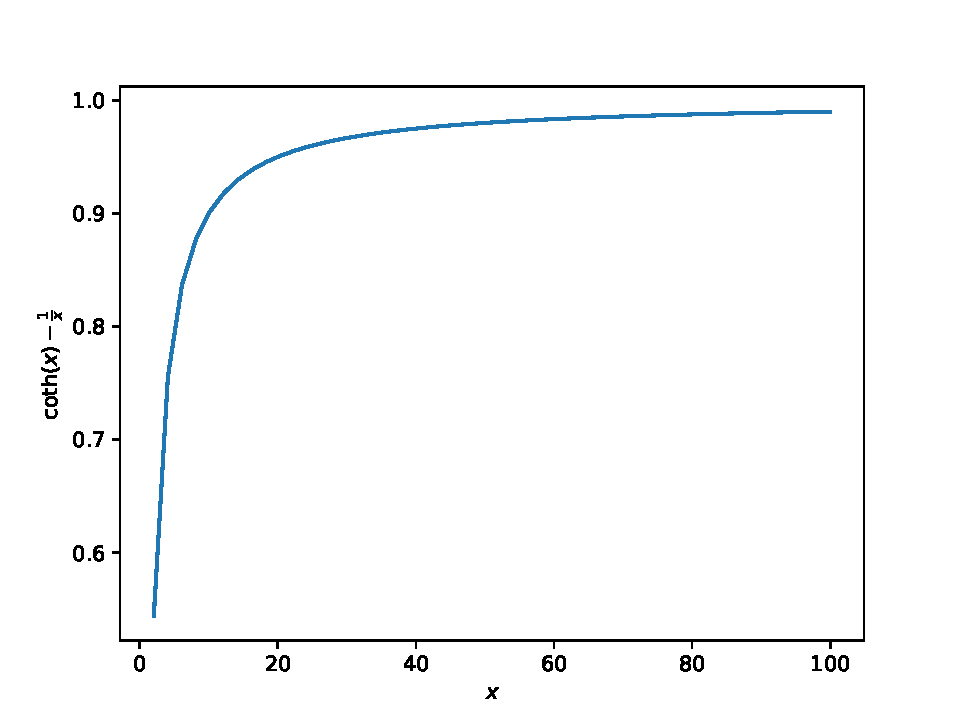
\includegraphics[width=.6\textwidth]{./figures/magnetization.pdf}
    \end{figure} \ \\ 

\paragraph{3. Discuss the two limiting cases: 
    high temperature/weak field vs. 
    low temperature/strong field.
    \textit{(2 points)}
} \ \\
    \\
    For $T\to0, M\sim N\mu$. \\
    For $T\to\infty, M\sim\frac{1}{2}N\mu(\beta\mu h)=\frac{1}{2}N\beta\mu^2 h\to0$

    \newpage

    \section{Rigid rotator \textit{(8 points)}}
    Add this after tutorial!
    \newpage

    \section{Adsorption of molecules to a surface \textit{(7 points)}}
    In the lecture we have derived the following 
RG flow equation for the coupling constant $K$ 
of the Ising chain without magnetic field: 
the new value $K'$ is given by
\begin{equation}
    K'(K)=\frac{1}{2}\ln\cosh(2K).
\end{equation}
In addition we have derived the absolute 
increase in free energy per spin arising in 
each iteration:
\begin{equation}
    g(K)=\frac{1}{2}\ln2
    +\frac{1}{4}\ln\cosh(2K)
\end{equation}

\paragraph{1. Write a short computer program 
    (e.g. in Mathematica or Python) that 
    defines the flow equation $K'(K)$ and the 
    free energy increase $g(K)$ as functions. 
    Start with a coupling constant $K_0=1$ and 
    iterate through $K_1$, $K_2$, $K_3$ up to 
    $K_4$. Also calculated the corresponding 
    values $g_0=g(K_0)$ to $g_4=g(K_4).$ What 
    are the limits for these two series? 
    \textit{(1.5 points)}
} \ \\
    \\
    Python functions:
    \lstinputlisting[firstline=6, lastline=11]{./code/task03a.py}
    Iteration to $i=4$ yields
    \begin{table}[h!]
        \begin{center}
        \begin{tabular}{llllll}
                  & i=0  & i=1  & i=2  & i=3  & i=4  \\ 
            \hline
            $K_i$ & 1    & 0.66 & 0.35 & 0.11 & 0.01 \\ 
            $g_i$ & 0.68 & 0.52 & 0.4  & 0.35 & 0.35 \\ 
        \end{tabular}
        \end{center}
    \end{table} \ \\ 
    The $K_i$-series converges to zero for 
    large $i$, while the $g_i$-series 
    converges to $\frac{1}{2}\ln2\approx0.35$.
    \begin{figure}[h!]
        \centering
        \begin{minipage}{.5\linewidth}
          \centering
          \subfloat[coupling constant $K$]{
            \label{:a}
            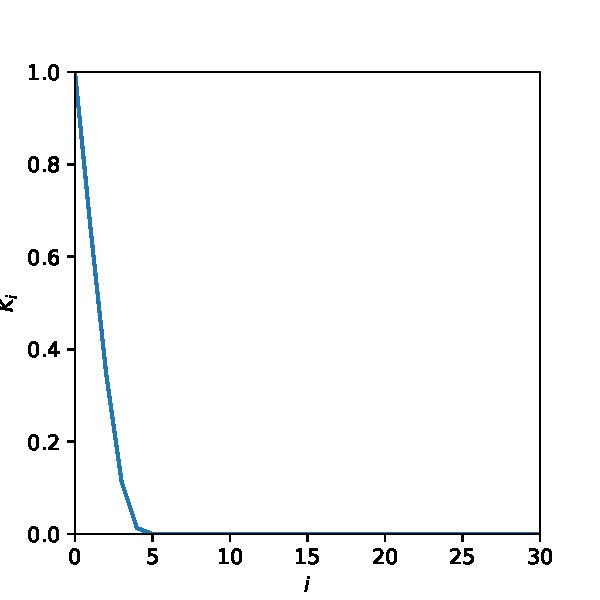
\includegraphics[scale=.7]{./figures/K_series.pdf}
          }
        \end{minipage}%
        \begin{minipage}{.5\linewidth}
          \centering
          \subfloat[free energy increase $g$]{
            \label{:b}
            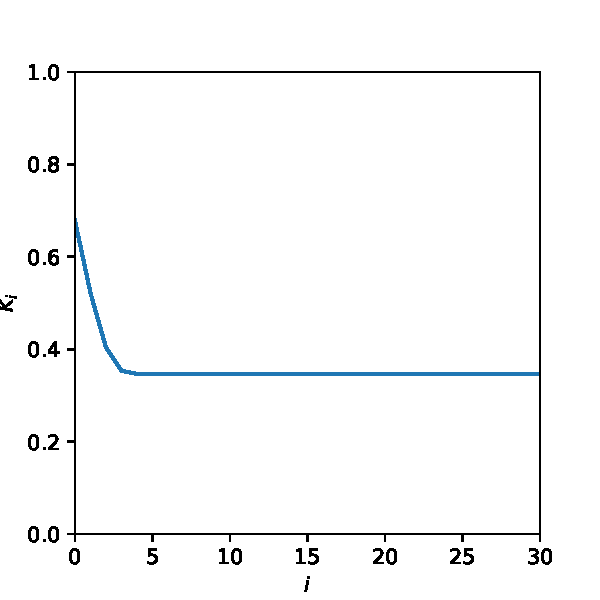
\includegraphics[scale=.7]{./figures/g_series.pdf}
          }
        \end{minipage}
    \end{figure} \ \\


\paragraph{2. Use these results to estimate 
    the dimensionless free energy per spin 
    $f=-\beta F/N$ in fourth order (simply cut 
    the appropriate sum after the term with 
    $g_4$; you can also include the next order
    term, but now by simply using the first 
    term in $g(K)$). Compare to the known 
    exact result for the Ising chain. How good
    is the numerical agreement?
    \textit{(1.5 points)}
}	\ \\
    \\
	Our result by summing the series for $g$:
    \begin{align}
        f
        &=\sum_{i=0}^{4} \frac{g_i}{2^i}
        \approx1.106 \,.
    \end{align}
    Compare to exact result $f=\ln\left(2\cosh(K)\right)=1.127$ for $K=1$.

    \newpage

    \section{Random walk \& self-avoiding random walk 
        \textit{(10 bonus points)}
    }
    In this exercise, we will write two small computer programs for random
walks on a $2D$ square lattice:
\begin{itemize}
    \item one for the usual random walk, where the walker is allowed to 
        come back to points already visited
    \item one for the so-called self-avoiding random walk (SAW), 
        where the walker is not allowed to do so and hence does not 
        cross its own path.
\end{itemize}
HINT: One can find a lot of algorithms for the SAW in the web. It is ok 
to use just the simplest one: When the walker revisits a position, you 
discard the walk. Otherwise you use the trajectory. Note that this 
algorithm for the SAW is not very efficient (you have to reject more 
and more trajectories for larger $n$), so you should restrict yourself 
to $n<N$ with, say, $N=30$. For the usual random walk there is no such 
problem and you can explore larger $N$.

\paragraph{a) Write the program for a typical RW} \ \\
\\
    The code for a non-self-avoiding random walk is pretty 
    straight-forward: At each step, we randomly choose an axis along
    which we will move ($x$ or $y$), and then choose a random 
    number from the set $\{-1, +1\}$ to get the direction along the 
    chosen axis:
    $y$-direction, respectively. \\
    \begin{code}{calc\_random\_walk\_trajectory.py}
        import numpy as np
        
        
        def main(nr_of_steps, x=0, y=0):
        
            def random_step(x, y):
                direction = np.random.choice(['x', 'y'])
                if direction == 'x':
                    dx = np.random.choice([-1, 1])
                    dy = 0
                elif direction == 'y':
                    dx = 0
                    dy = np.random.choice([-1, 1])
        
            trajectory = []
            for i in range(nr_of_steps):
                x, y = random_step(x, y) 
                trajectory.append((x, y))
        
            return trajectory\end{code} \ \\
    \noindent
    It was not entirely clear from the formulation in the problem set 
    whether diagonal steps are allowed as well. 
    Including them would lead to the step size not being constant 
    (sometimes being $1$, sometimes $\sqrt{2}$). If one wishes to 
    allow diagonal steps as well, one could simply adjust the 
    \lstinline{random_step} method like this: \\
    \begin{code}{calc\_random\_walk\_trajectory.py}
        def random_step(x, y):
            dx = np.random.choice([-1, 0, 1])
            dy = np.random.choice([-1, 0, 1])
            return x+dx, y+dy\end{code}

\newpage
\paragraph{b) Write the program for a SAW} \ \\
\\
    To make the random walk self-avoiding, we simply have to check 
    at each step whether or not the position of the next step has 
    already been reached at an earlier time. If it has, we just return 
    \lstinline{None} instead of the trajectory. Outside of
    \lstinline{calc_random_walk_trajectory} in the 
    \lstinline{main} function, we run a 
    \lstinline{while} loop, which repeats the function execution until a 
    non-\lstinline{None} value has been returned.
    \begin{code}{calc\_random\_walk\_trajectory.py}
        import numpy as np
        
        
        def main(nr_of_steps, self_avoiding=True, x=0, y=0):
        
            def random_step(x, y):
                direction = np.random.choice(['x', 'y'])
                if direction == 'x':
                    dx = np.random.choice([-1, 1])
                    dy = 0
                elif direction == 'y':
                    dx = 0
                    dy = np.random.choice([-1, 1])
                return x+dx, y+dy

            trajectory = []
            for i in range(nr_of_steps):
                x, y = random_step(x, y)
        
                if self_avoiding and (x, y) in trajectory:
                    return None
        
                trajectory.append((x, y))
        
            return trajectory\end{code}

    \begin{code}{main.py}
        from calc_random_walk_trajectory import main as calc_random_walk_trajectory
        
        
        def main(nr_of_steps=30, self_avoiding=True):
        
            trajectory = calc_random_walk_trajectory(nr_of_steps, self_avoiding)
            if self_avoiding:
                while trajectory is None:
                    trajectory = calc_random_walk_trajectory(
                        nr_of_steps, self_avoiding
                    )
        
            filename = 'SAW' if self_avoiding else 'RW'
            plot_trajectory(trajectory, nr_of_steps, filename)\end{code}

\newpage
\paragraph{c) Show some representative trajectories.} \ \\
\\
    Without diagonal steps:
    \begin{figure}[h!]
        \centering
        \begin{minipage}{.5\linewidth}
          \centering
          \subfloat[normal random walk ($n=400$)]{
            \label{:a}
            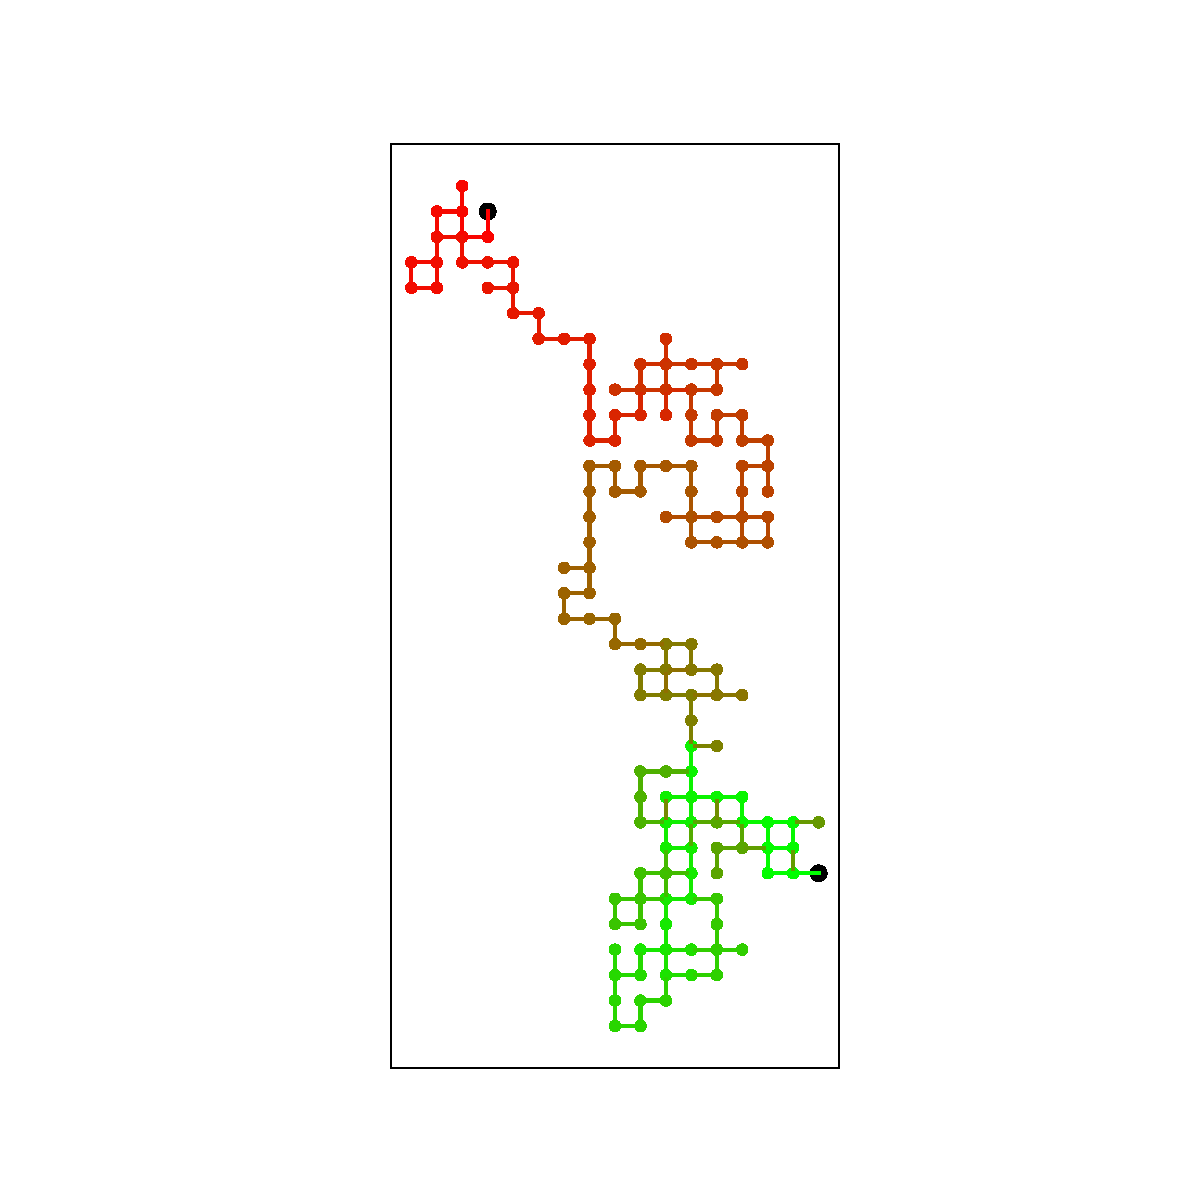
\includegraphics[scale=.45]{./figures/RW.pdf}
            % 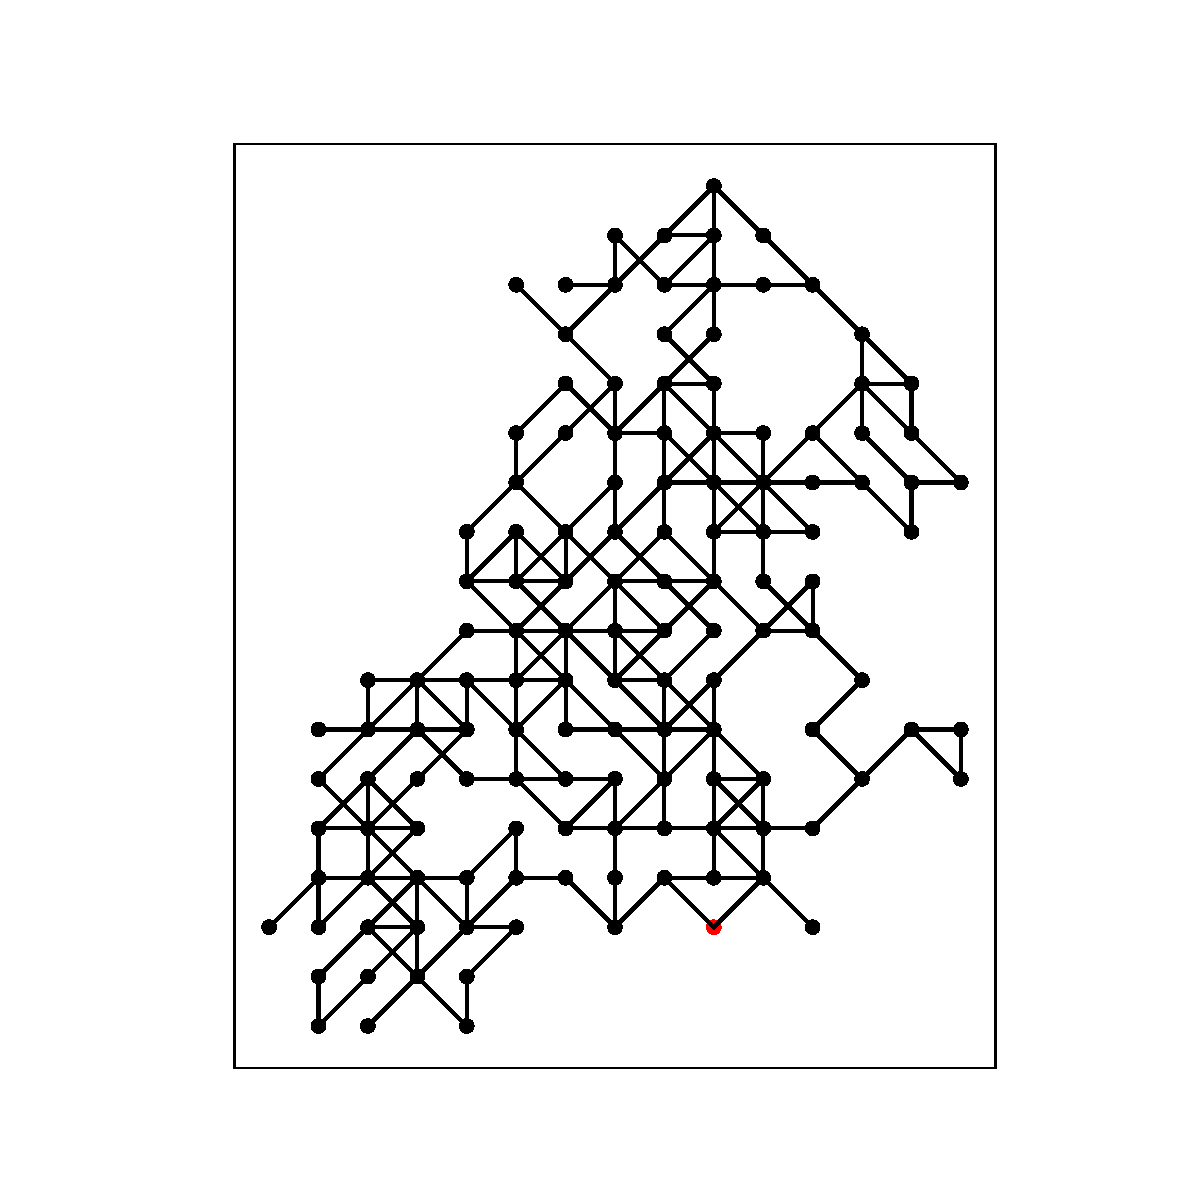
\includegraphics[scale=.5]{./figures/RW_good.pdf}
          }
        \end{minipage}%
        \begin{minipage}{.5\linewidth}
          \centering
          \subfloat[self-avoiding random walk ($n=30$)]{
            \label{:b}
            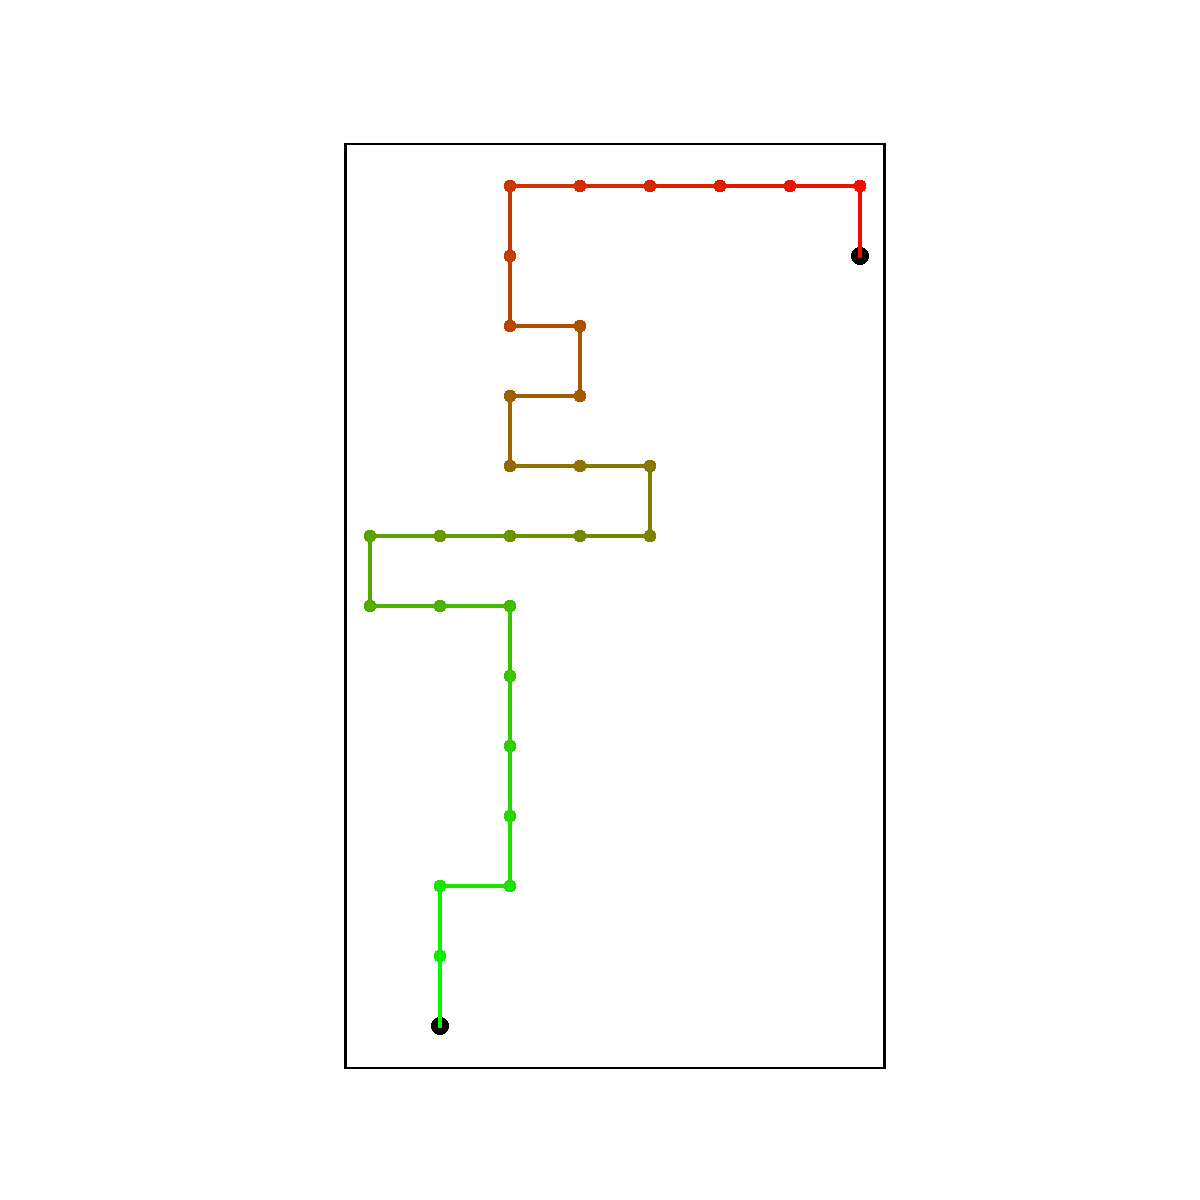
\includegraphics[scale=.45]{./figures/SAW.pdf}
            % 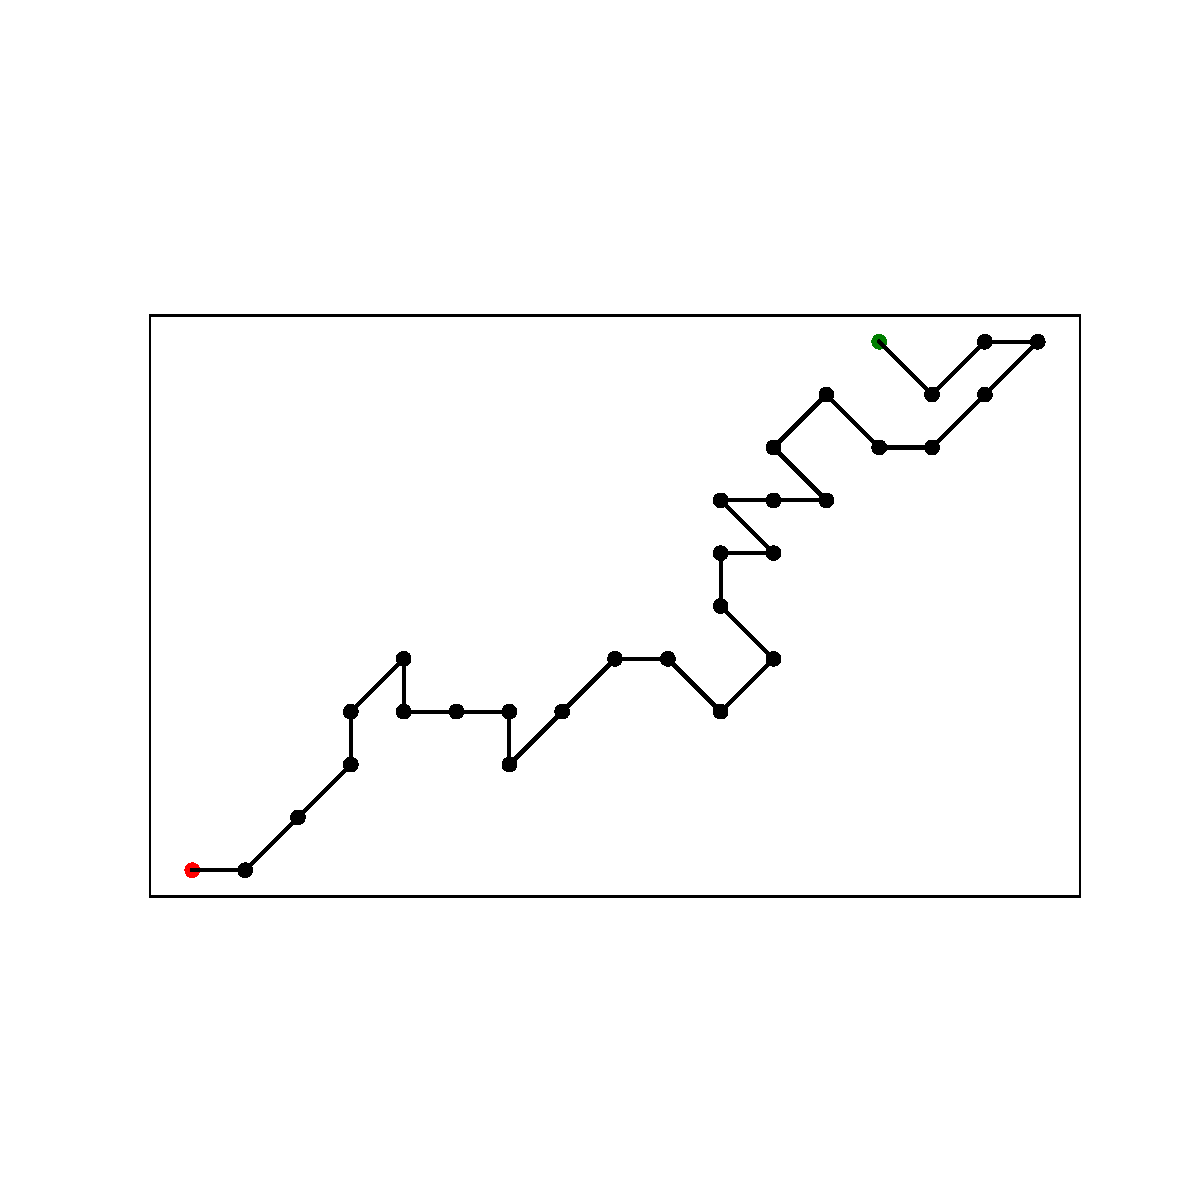
\includegraphics[scale=.5]{./figures/SAW_good.pdf}
          }
        \end{minipage}
    \end{figure} \ \\
    With diagonal steps:
    \begin{figure}[h!]
        \centering
        \begin{minipage}{.5\linewidth}
          \centering
          \subfloat[normal random walk ($n=400$)]{
            \label{:a}
            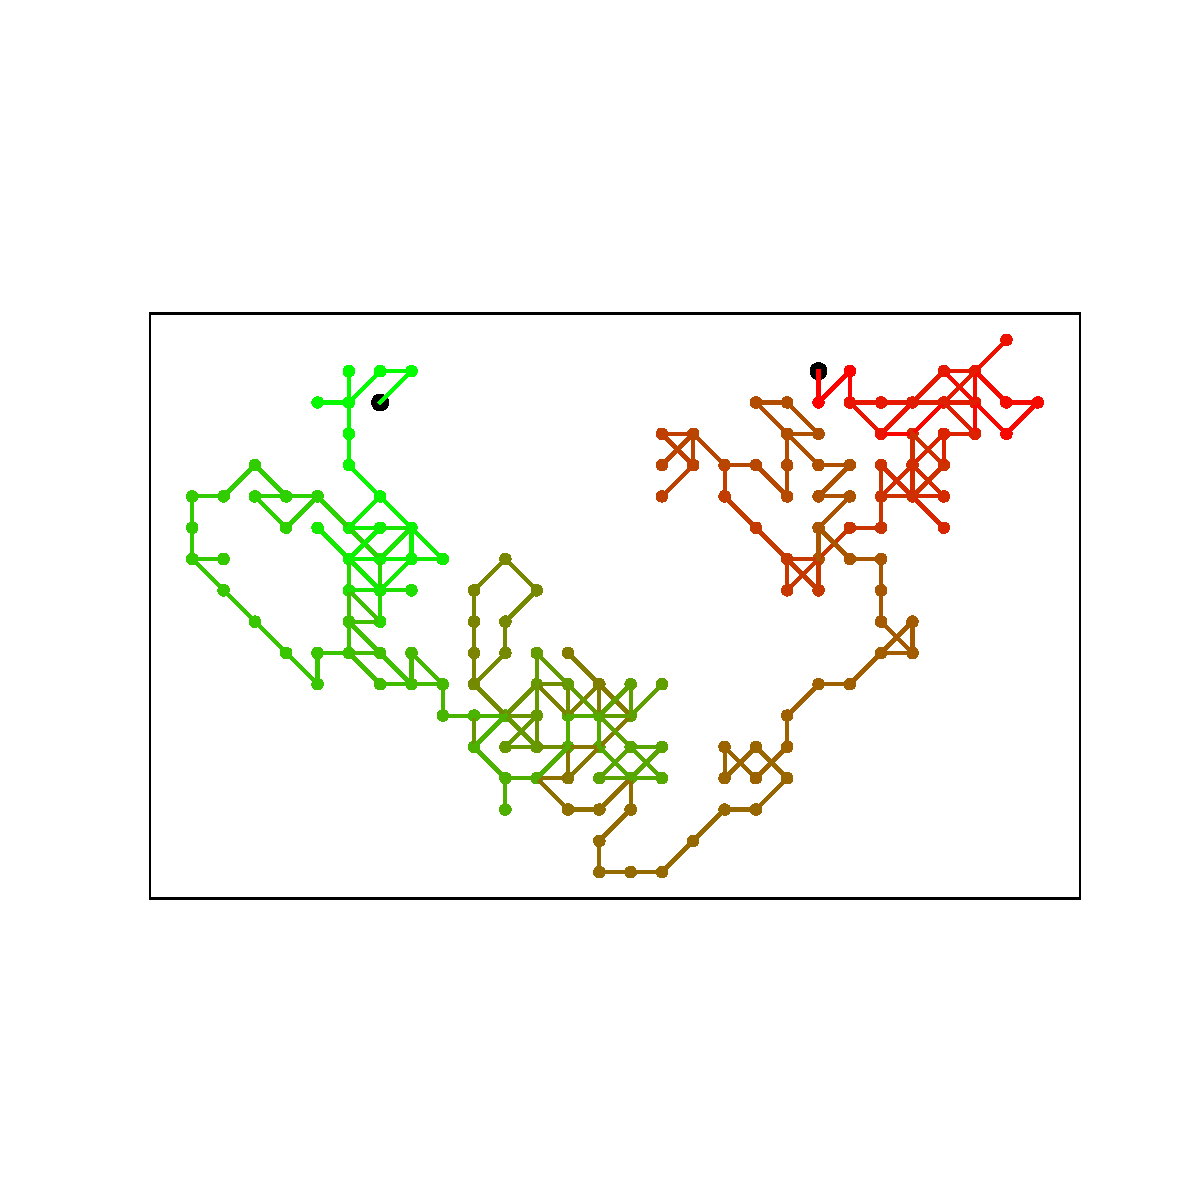
\includegraphics[scale=.45]{./figures/RW_diag.pdf}
            % 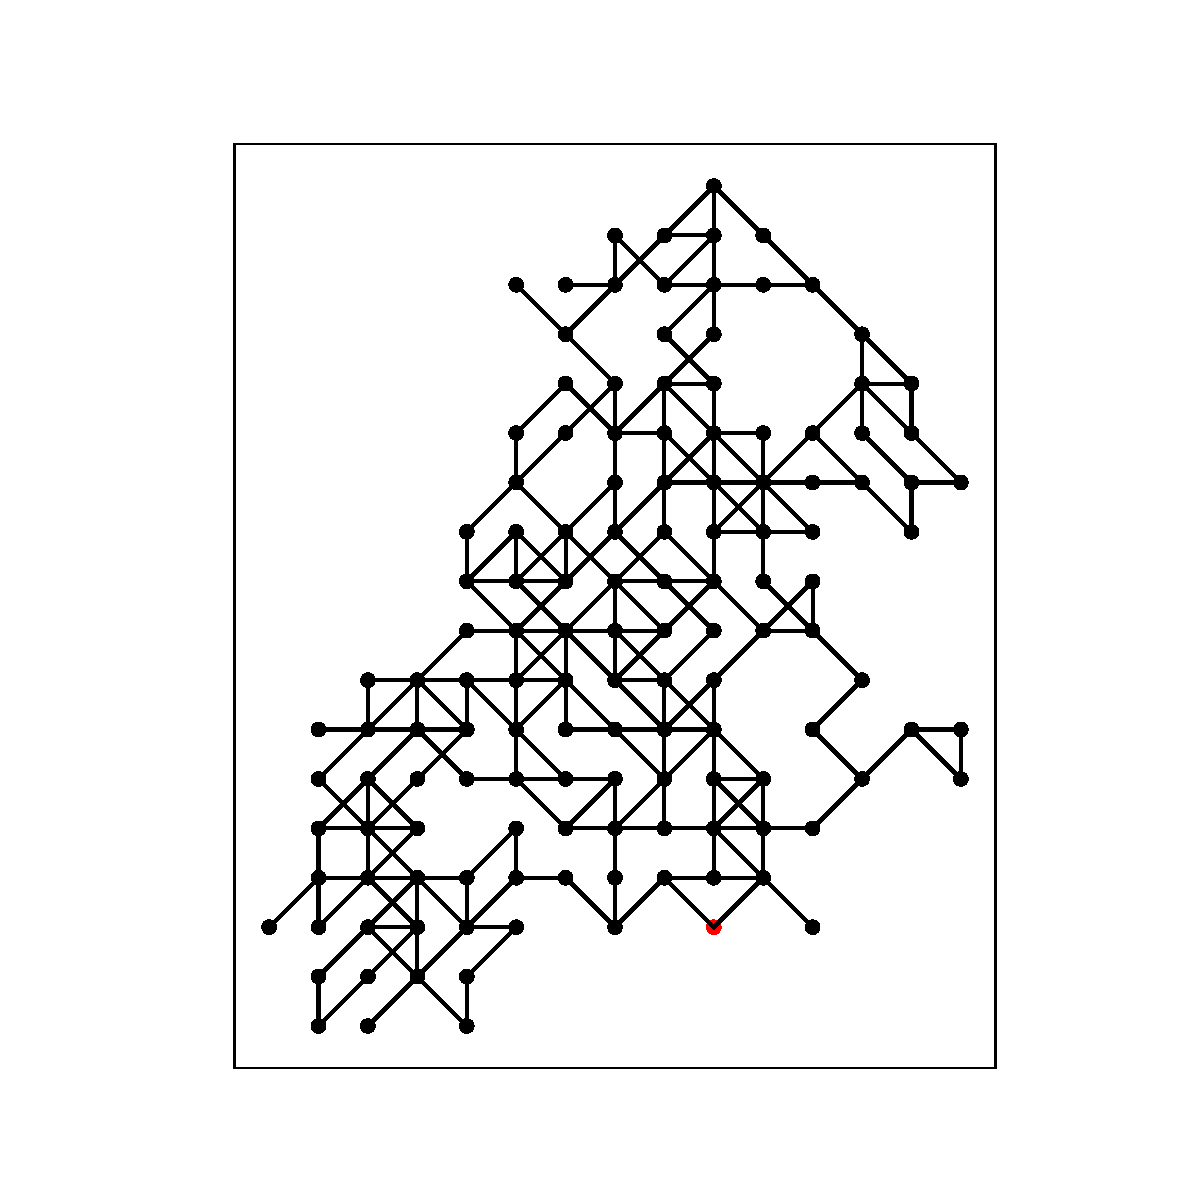
\includegraphics[scale=.5]{./figures/RW_good.pdf}
          }
        \end{minipage}%
        \begin{minipage}{.5\linewidth}
          \centering
          \subfloat[self-avoiding random walk ($n=30$)]{
            \label{:b}
            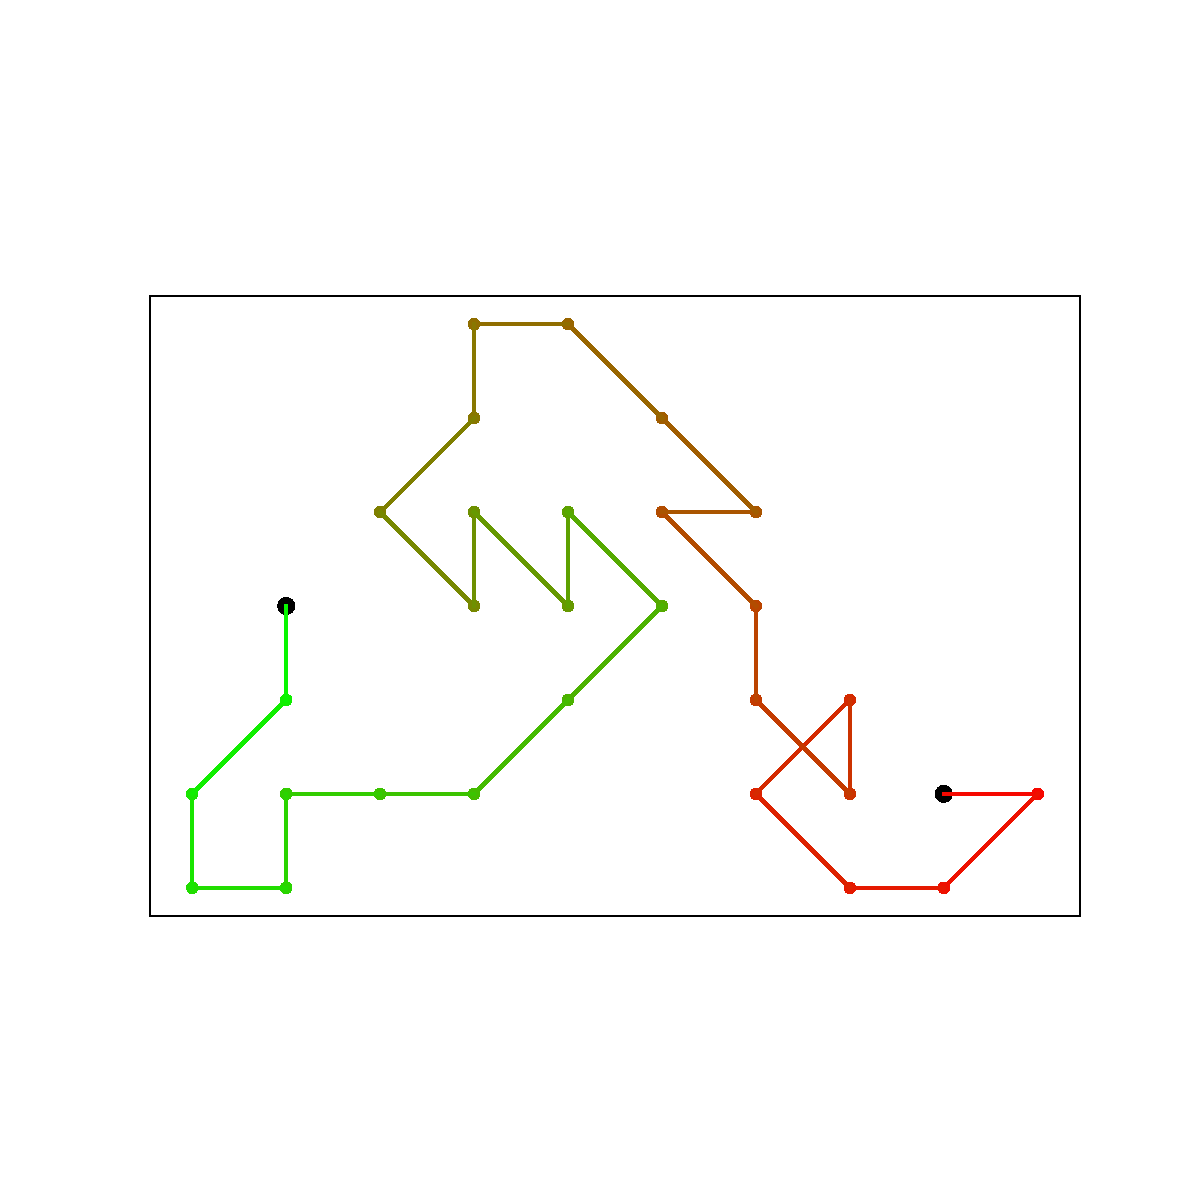
\includegraphics[scale=.45]{./figures/SAW_diag.pdf}
            % 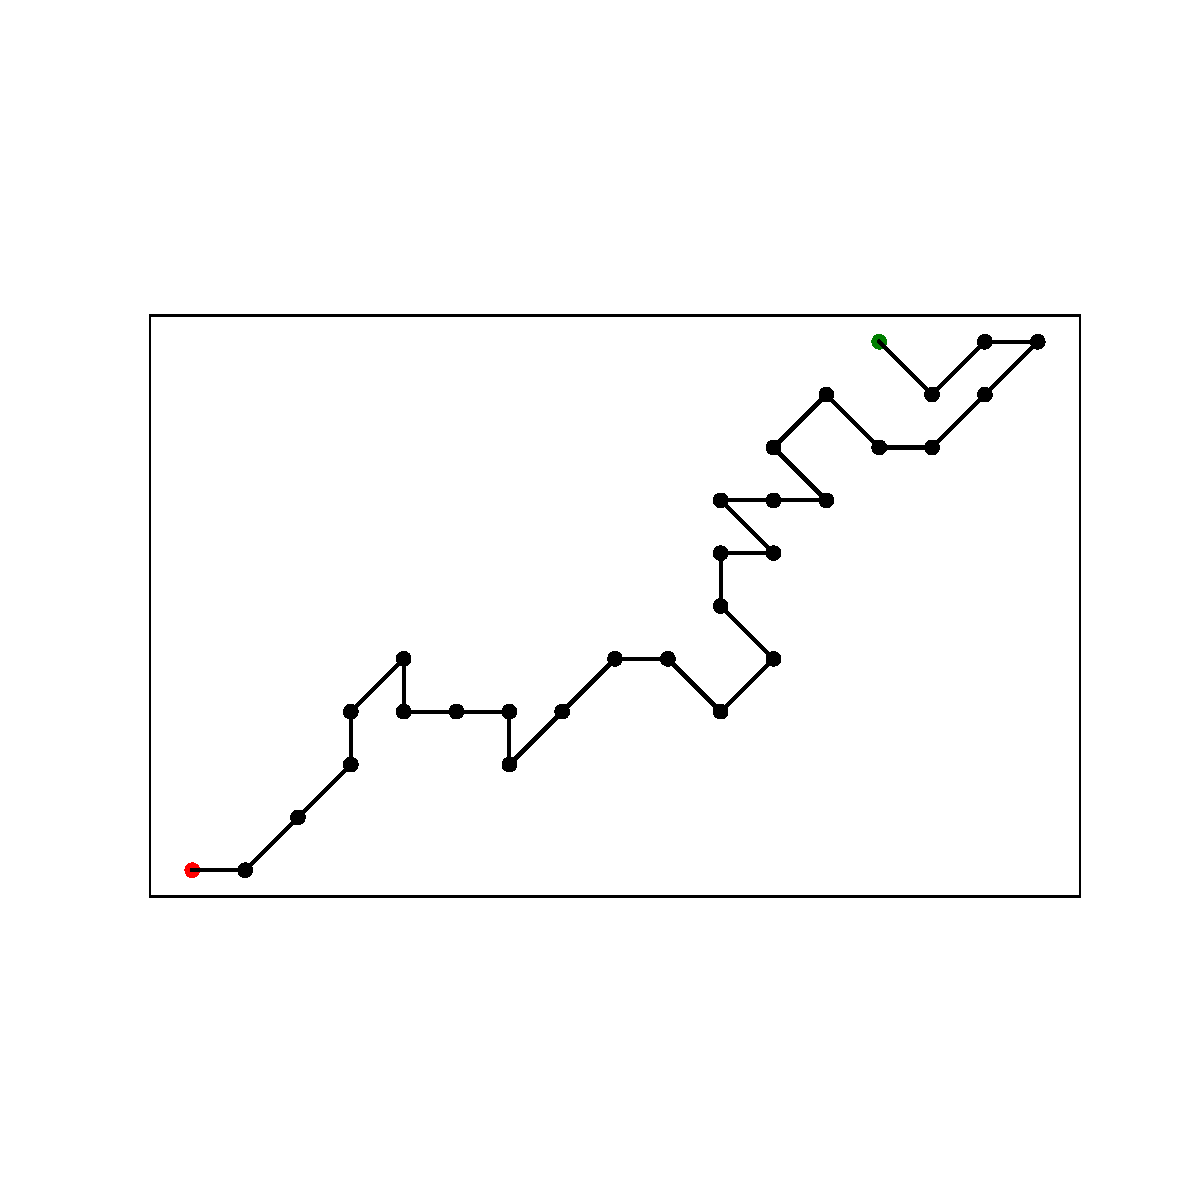
\includegraphics[scale=.5]{./figures/SAW_good.pdf}
          } 
        \end{minipage}
    \end{figure} \ \\

\newpage
\paragraph{d) Measure the mean squared displacements (MSD) 
    $\langle x^2(n)\rangle$ as a function of the number of steps $n$ 
    for both cases (the average is over different trajectories). If you 
    plot the results in log-log-scale you can extract the exponents 
    $\alpha$, where $\langle x^2(n)\rangle\sim n\alpha$, for the two 
    cases. Compare and discuss.
} \ \\
\\
    To get the average over different trajectories, for each number of 
    steps we calculate 100 trajectories (in this case, without 
    allowing diagonal steps), then we calculate the squared 
    displacements for each of the trajectories and take the mean.
    Then, we plot this in a linear fashion: \\
    \begin{figure}[h!]
        \centering
        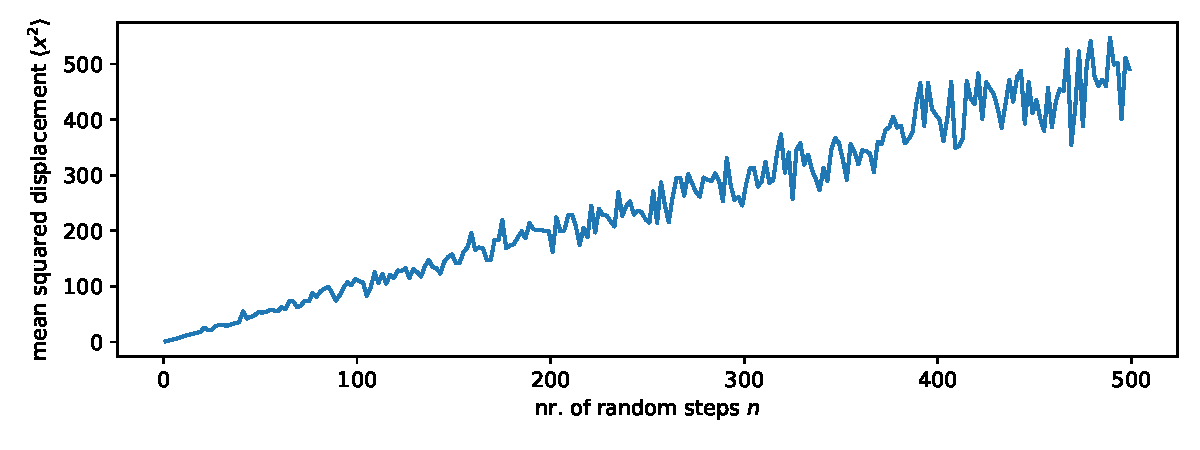
\includegraphics[width=\textwidth]{./figures/MSD_vs_N.pdf}
        \caption{mean squared displacement as a function of steps}
    \end{figure} \ \\
    \\
    And now as a log-log plot: \\
    \begin{figure}[h!]
        \centering
        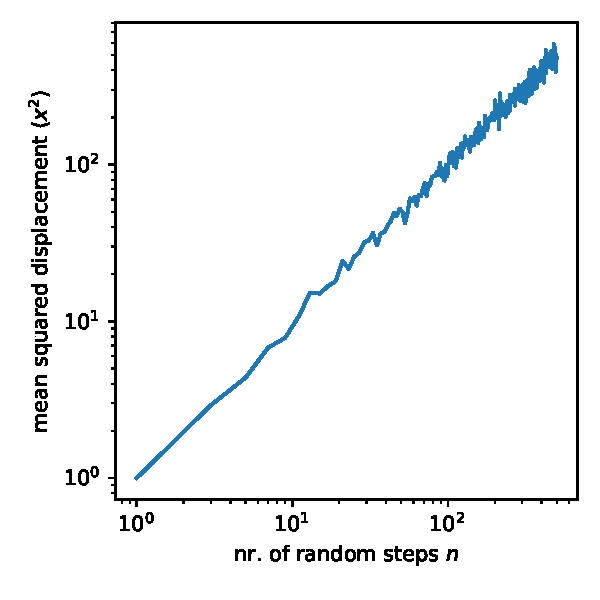
\includegraphics[width=\textwidth]{./figures/MSD_vs_N_loglog.pdf}
        \caption{mean squared displacement as a function of steps}
    \end{figure} \ \\
    \\




\end{document}
